%======================================================================
\subsection{BW-ROB-05 --- Built, 27 Oct: Drive Joint, Motion Study, Motion Link}\label{sec:rob05-built}
%======================================================================

The kinematic half of the motion epic (your decision of 27 Oct: kinematic first, dynamics later in
ASM-10) is built, in three commits (\code{c41cabc8}, \code{d8dc3727} and the roadmap commit), all Python in
\file{src/Mod/BruceWorx/bruceworx\_motion.py} on top of FreeCAD 1.1's kinematic Simulation (the Ondsel
solver through \code{assembly.generateSimulation}). Nothing in C++ changed.

\begin{figure}[!htbp]
\centering
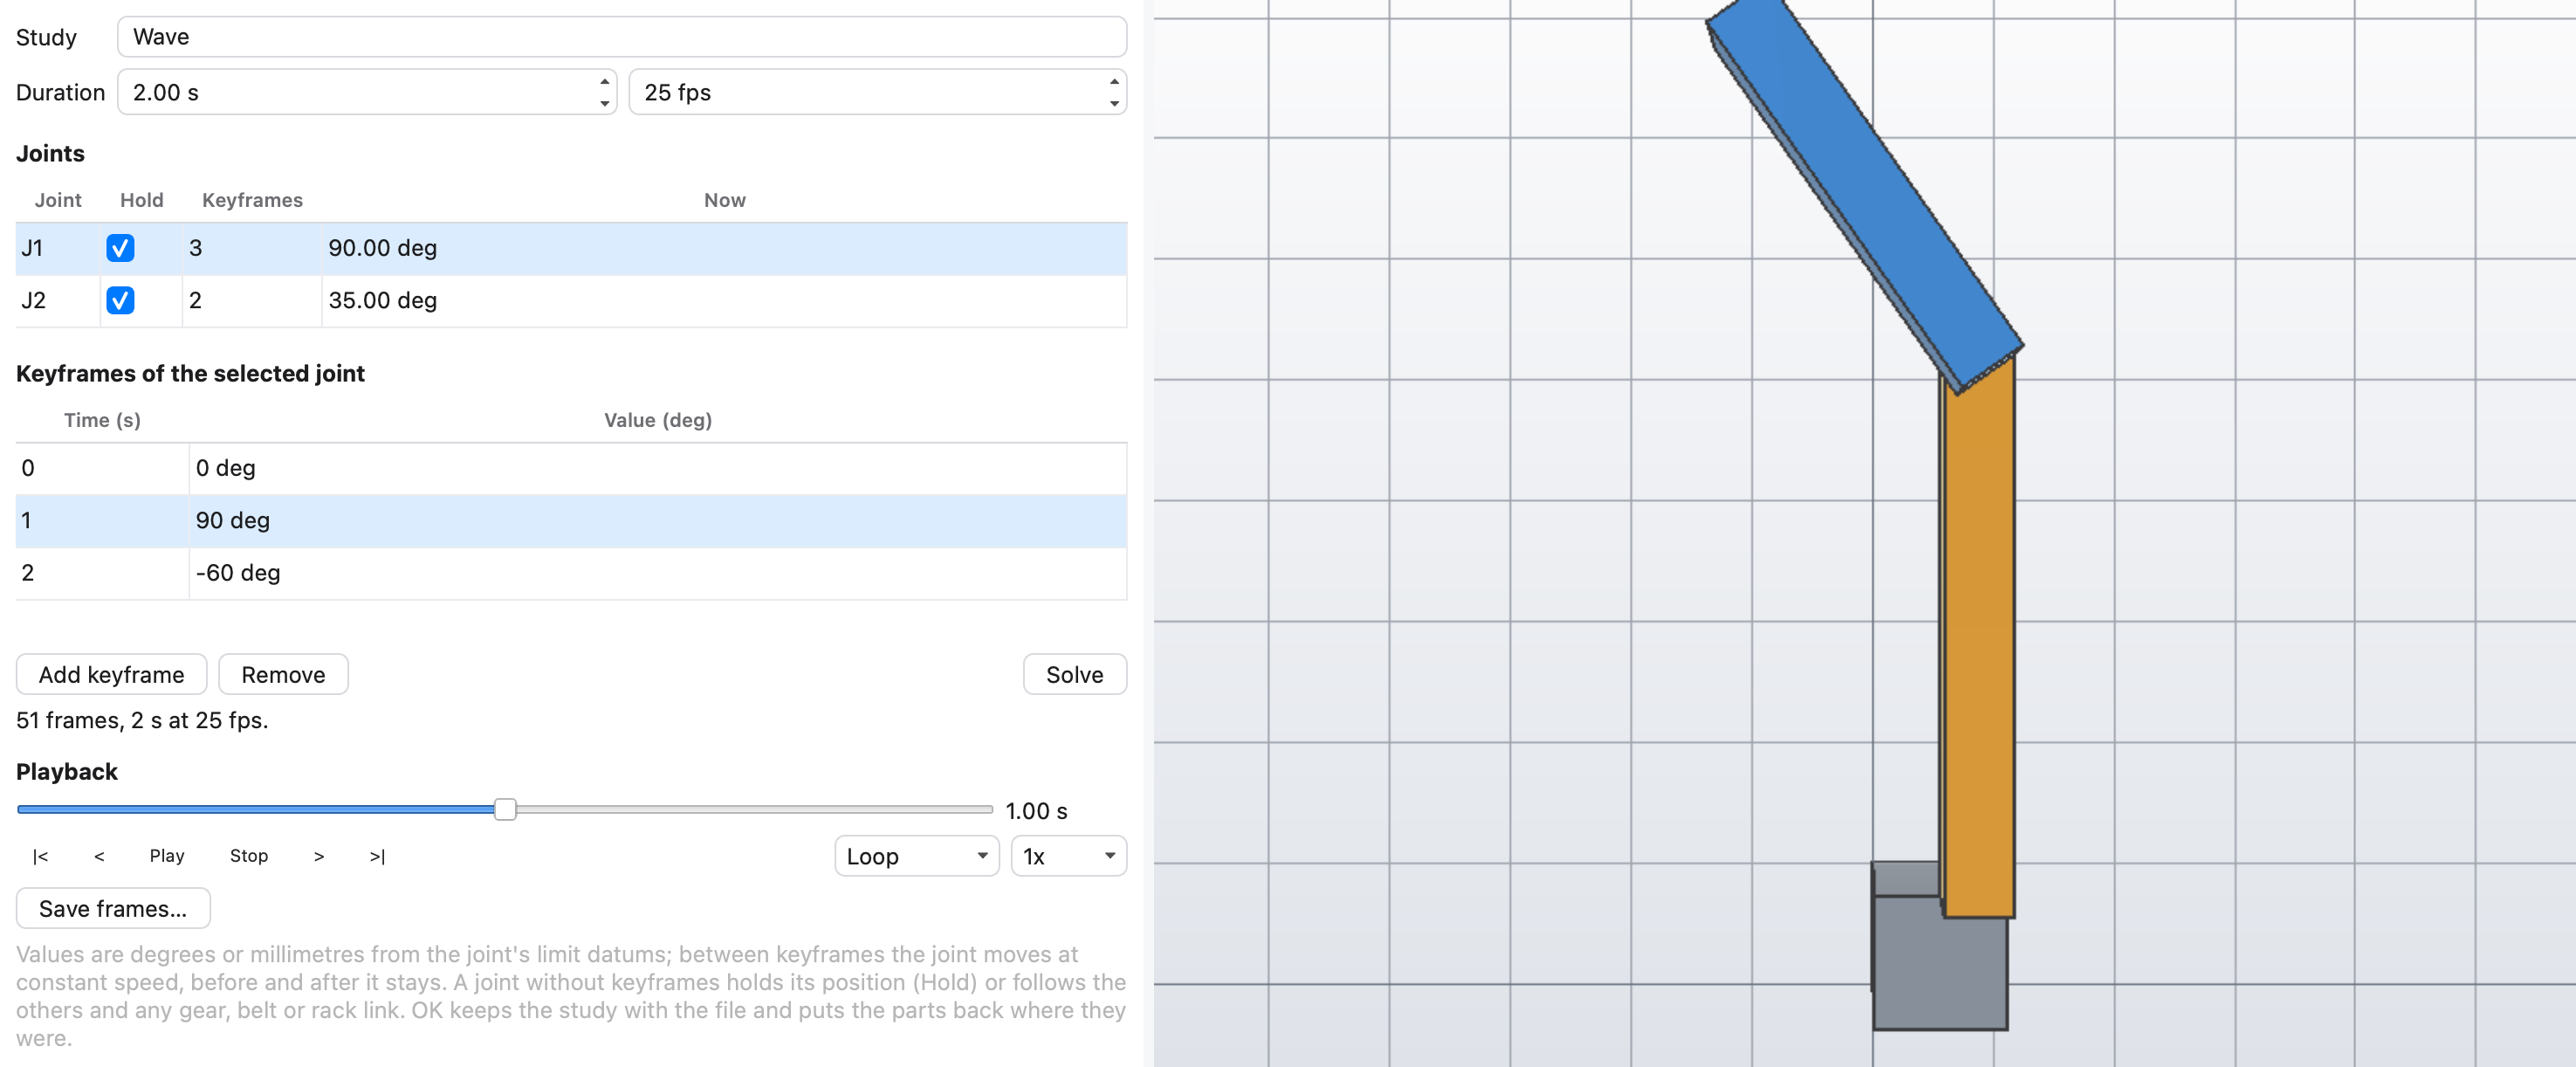
\includegraphics[width=\linewidth]{fig/motion_study.png}
\caption{The Motion Study panel on the 2-DOF test arm at $t = 1$\,s: the joints with their keyframe
counts and present readings, the keyframes of J1 with the one at the current time highlighted, the scrub
slider, playback mode and speed, and Save frames. Right: the arm at that frame (J1 at $90^\circ$, J2 at
$35^\circ$ between its keyframes at 0.5 and 1.5\,s).}
\label{fig:rob05-study}
\end{figure}

\paragraph{What is on the ribbon now.}
\begin{itemize}[nosep]
  \item \textbf{Joint}, in the Assemble group: one button whose menu lists all thirteen joint types with
        their own icons (fixed, revolute, cylindrical, slider, ball, distance, parallel, perpendicular,
        angle, rack and pinion, screw, gears, belt). Revolute and Slider stay beside it as before; Fixed
        moved into the group's more list, and the ten joint commands that were only in that list are gone
        from it (they are in the menu).
  \item \textbf{Motion}, a new group after Assemble: Drive Joint, Motion Study, Motion Link, with
        FreeCAD's own Simulation command in its more list.
\end{itemize}

\paragraph{Drive Joint.} A combo of the assembly's drivable joints (revolute, slider, cylindrical with an
angle and a length row, screw), a slider and a spin box over the joint's range: its limits when both are
set, otherwise $-180\ldots180^\circ$ or $-100\ldots100$\,mm. The model follows live; the other joints
stay where they are, and a joint coupled by a gear, belt or rack joint follows the drive. Animate sweeps
the range back and forth at the speed given (deg/s or mm/s). OK keeps the pose as one undo step
(``Drive joint''); Cancel puts every part back and leaves no object in the file, not even the
Simulations group when the panel made it.

\paragraph{Motion Study.} The study is a Simulation object (\code{CommandCreateSimulation}'s class, so
FreeCAD's own panel opens it too) with one Motion per joint channel. Its panel has the duration and frame
rate, the joints table (Hold, keyframe count, the reading at the shown frame), the keyframes of the
selected joint (time in s, value in deg or mm, editable in place, Add at the current time with the current
value, Remove), Solve, a scrub slider with the time, $|\!<$, $<$, Play/Pause, Stop, $>$, $>\!|$, Once /
Loop / Ping-pong, $0.25\times$ to $4\times$, and Save frames, which writes \file{frame\_0001.png}\ldots at
$1280\times720$ and \file{motion.mp4} when ffmpeg is on the PATH. OK keeps the study with the file and puts
the parts back where they were (as FreeCAD's panel does); Cancel undoes the edit and removes a new study.

\paragraph{Motion Link.} Two joints and a ratio become the stock joint that couples them: two revolutes a
Gears joint (the follower turns the other way; Reverse makes it a Belt, same way), a revolute and a slider
a Rack and Pinion with the travel per turn (Reverse flips the sign of the pitch radius). The joint is
labelled \code{Link: J1 -> J3 (1:3)} or \code{(36 mm/turn)}. Two sliders are refused with the reason: the
solver has no joint for them.

\begin{figure}[!htbp]
\centering
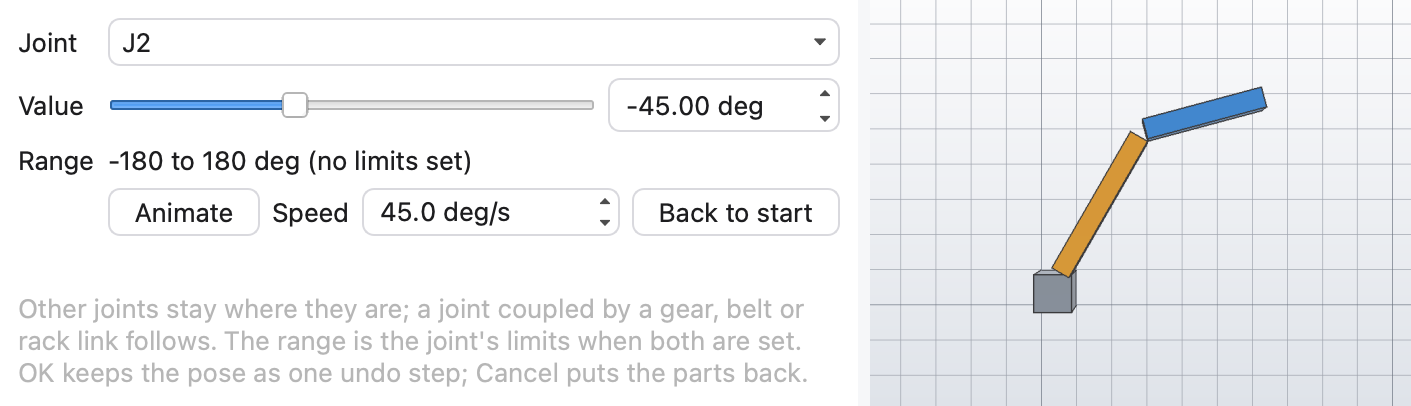
\includegraphics[width=0.66\linewidth]{fig/motion_drive.png}\hfill
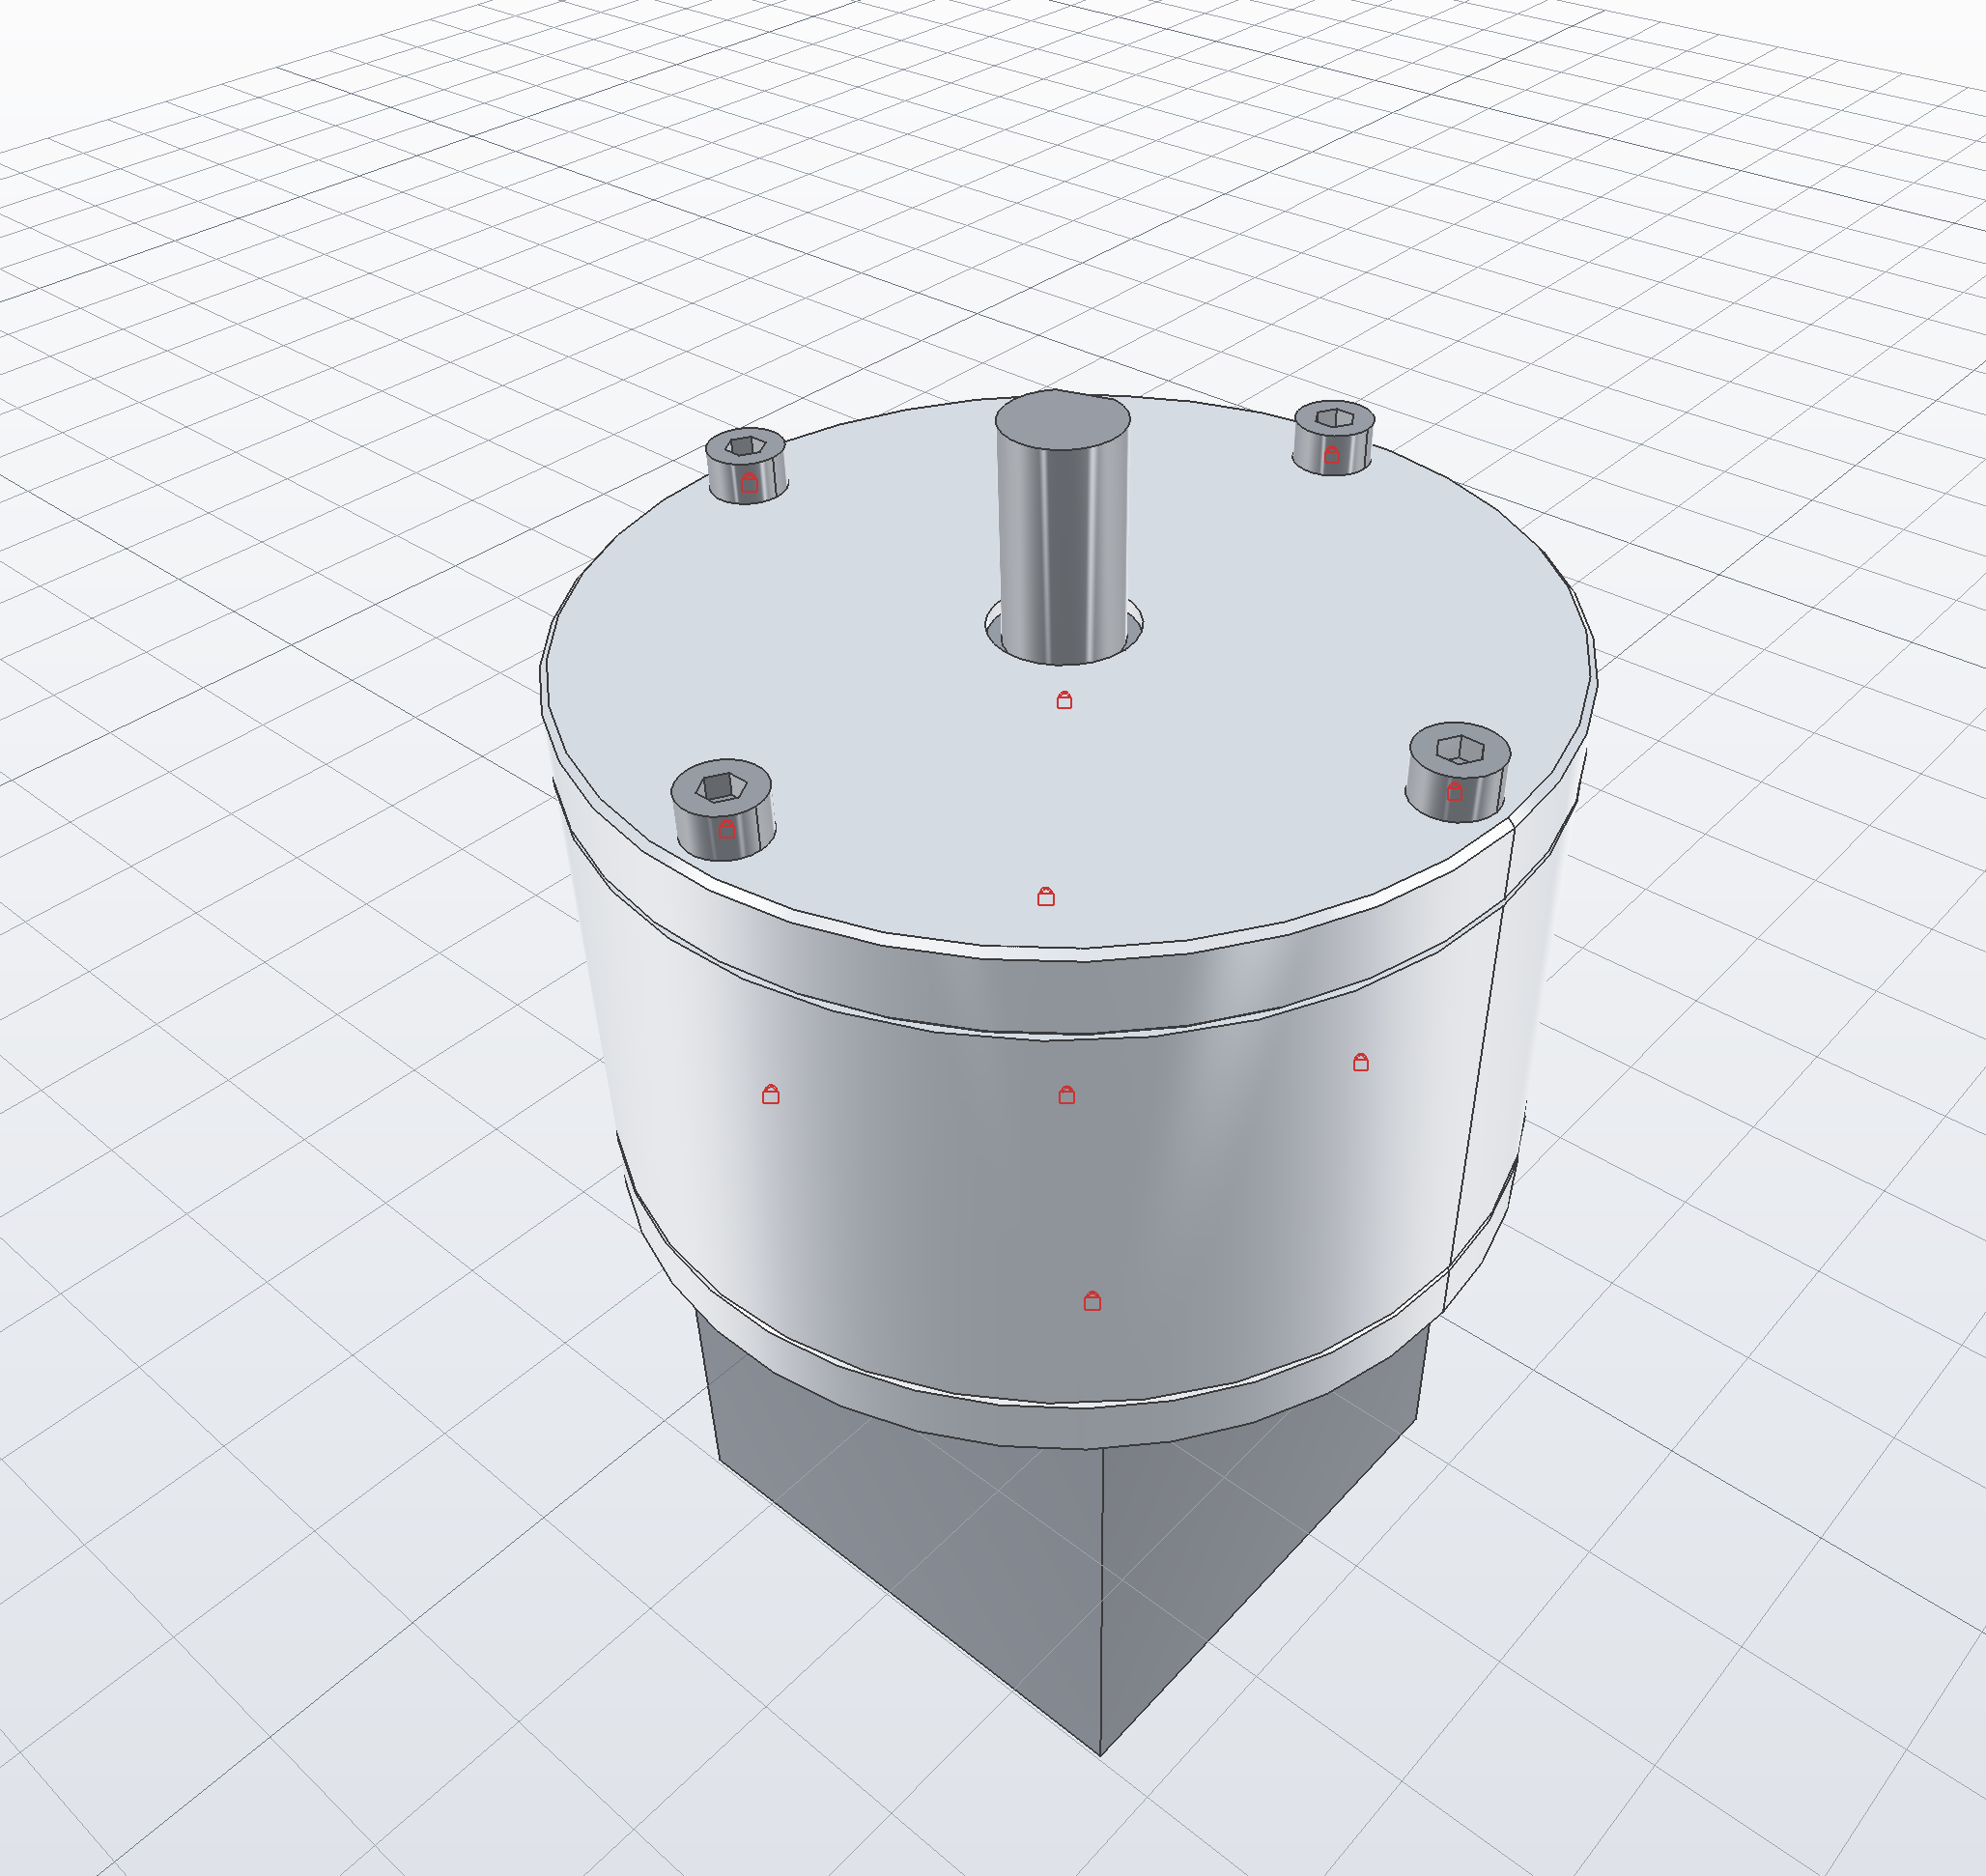
\includegraphics[width=0.32\linewidth]{fig/motion_gearbox.png}
\caption{Left: Drive Joint on J2 of the arm at $-45^\circ$ after J1 was put at $60^\circ$. Right: a copy of
the NEMA 17 planetary gearbox from the vault with its sun driven a quarter turn through the same panel
(carrier at $18^\circ$: the 5:1 of a 6/24 planetary, through the six Gears and Belt mesh joints already in
the file).}
\label{fig:rob05-drive}
\end{figure}

\paragraph{Decided while building.}
\begin{itemize}[nosep]
  \item \textbf{The solver, not the drag API.} The brief left the choice. In a spike the drag API moved a
        two-link chain nowhere when its first link was turned (the solver pulls the dragged part back
        when a second part hangs on it), and it cannot hold the other joints. A Simulation with a
        constant formula per joint is exact and holds everything else, so Drive Joint runs one, inside its
        own transaction, and removes it on OK or Cancel. On the gearbox copy a drive step takes 36\,ms.
  \item \textbf{Keyframes compile to \code{piecewise()}.} Tested headless first: the parser takes
        \code{piecewise(time, functions(f0, f1, \ldots), transitions(t0, t1, \ldots))}, angles in
        radians, lengths in mm, and its frame 0 is the start pose (frames 1\ldots$n$ are $t_0$ to $t_{end}$).
        A joint's keyframes are the source of truth, on the Motion as \code{BWKeyframes}; the Formula is
        derived (constant before the first and after the last, linear between). Values are readings from
        the joint's limit datums (\S\ref{sec:joints}), so the datum zero is put back in the formula.
  \item \textbf{A joint without keyframes holds} its position, as Fusion's studies do, through a constant
        Motion; the Hold column turns that off. A joint whose part is coupled by a Gears, Belt, Rack and
        Pinion or Screw joint starts with Hold off, so the gearbox's carrier and planets follow the sun
        instead of fighting it.
  \item \textbf{Big moves go in steps of $60^\circ$.} Found in the GUI tests: the solver's rotational
        motion has a second solution $180^\circ$ away, and a jump past $90^\circ$ lands on it ($90^\circ$
        to $-45^\circ$ came out as $135^\circ$). Drive Joint and the study's settling on its first
        keyframes now move in steps, the short way round; a study also runs from the pose it was opened
        in, since a run that begins far from its first keyframe may not converge at all.
  \item \textbf{Motion Link needs a shared carrier.} The gear constraint relates the orbit angles of the
        two gear centres in each other's frame, so it links two parts that turn on the same third part
        (sun and planet on the carrier); a chain (J2 on J1's arm) is not a gear relationship, and the
        solver simply holds it. The panel says so. Radii are 10\,mm and $10\times$ratio (edit the joint's
        Distance for real gears); a rack's pitch radius is travel$/2\pi$.
  \item \textbf{Cancel cleans up itself.} Aborting the transaction alone left the Simulations group
        behind (and does nothing headless), so Drive Joint and a new study remove their objects first.
  \item \textbf{One Motion per channel}, a cylindrical joint being two rows (angle, length) and a screw one
        (angle; the length follows the pitch).
\end{itemize}

\paragraph{Tests.} Headless (\file{AssemblyTests/TestBWMotion.py}, 16 tests): the interpolation and the
formula text, the 2-DOF arm reaching every keyframed pose at $t = 0, 0.25, \ldots, 1$\,s to $10^{-3}$
degrees, hold and follow, a suppressed joint dropped from a study, the Driver moving one joint while the
other stays, a $215^\circ$ jump in steps and $20^\circ$ the short way, Cancel leaving nothing and OK as one
undo step, gears driving the second joint at $-3\times$, a belt at $+0.5\times$, a rack at 36\,mm per turn
and reversed; the Assembly suite is at 41 passing (2 skipped) with \code{TestBWJoints} unchanged. GUI
(\file{src/Mod/BruceWorx/TestBruceWorxMotion.py} under \file{run\_gui\_tests.py}, 16 tests, 2.9\,s): the
menu's thirteen entries with icons, the Motion group's place, the slider moving the arm and Cancel putting
it back, OK as one undo step, limits bounding the slider, Animate bouncing at $180^\circ$; the study's
keyframes, solve, scrub with the highlighted keyframe, Once/Loop/Ping-pong, $4\times$, Hold off, five
frames and an MP4 written, Cancel of a new study and OK keeping it; Gears and Belt links, the same joint
twice refused. The \code{slot()} lint (\code{TestBruceWorx}, 15), Workspaces (25) and Groups (13) pass.
Real check: the gearbox copy (\file{LE-02-01002-001} and its parts, copied from the vault) runs a full sun
turn in 21 frames in 0.12\,s with the carrier at $72^\circ$ (5:1).

\paragraph{Not done.} The user-facing run inside your Keystone (the main session restages). A study
chooser: the command opens the latest study of the assembly or makes a new one. Keyframe easing (the solver
also offers \code{spline} and \code{rampstep}). A dynamics study (ASM-10).

\paragraph{Open questions for you.}
\begin{enumerate}[nosep]
  \item \textbf{Joint button.} Keep Revolute and Slider beside it on the ribbon, or the menu alone?
  \item \textbf{Several studies per assembly.} A chooser in the panel (combo, New), or is one study per
        assembly enough for now?
  \item \textbf{Gear radii.} The link writes 10\,mm and $10\times$ratio. Prefer to ask for module and
        teeth (or the two pitch radii) so the joint matches the drawn gears?
  \item \textbf{Easing.} Linear between keyframes, as built; want ease-in/out per keyframe?
  \item \textbf{Drive Joint and limits.} The slider stops at the limits and the solver's limit constraints
        hold too; the drag backstop of \S\ref{sec:joints} is not used. Fine, or should dragging in the
        panel feel exactly like the mouse drag?
\end{enumerate}
